\section{Theory} \label{tex:theory}
In this section, the theory used to develop the methods and obtain the result in this thesis will be discussed. First, neural networks (NNs) will be covered - both the simpler artificial NNs (ANNs) and more complex networks such as the convolutional NN (CNN) in both 2 and 3 dimensions. Also methods for calculating the theoretical speed of a NN will be covered. This is followed by the theory behind different methods in tensor decomposition, and how to choose the appropriate rank in some cases.
\begin{figure}[H]
    \centering
    \captionsetup{width=.95\linewidth}
    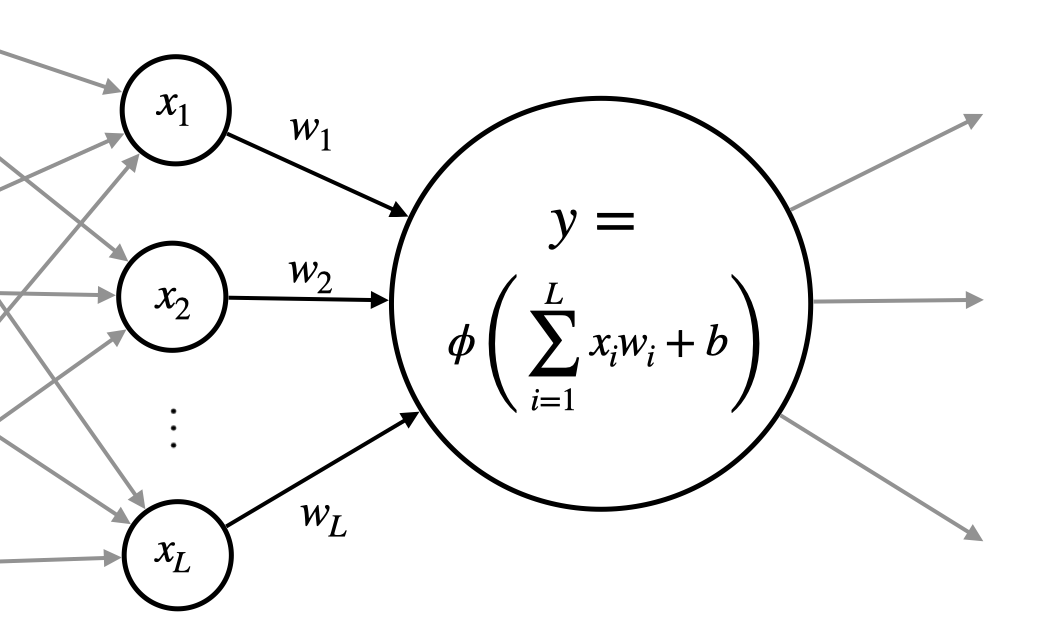
\includegraphics[width=.7\linewidth]{Pics/02_Theory/activation_illustration.png}
    \caption{Illustration of the flow of information through a neuron. Each edge (arrow) has a weight $w$ associated with it, and each neuron (circle) has an activation associated with it. The activations correspond to the information that is passed through the network. $\phi$ is the activation function.}
    \label{fig:activation_illustration}
\end{figure}
\subsection{Neural Networks}\label{tex:theory_NN}
The NN gets its name from what gave rise to the idea of it around half a century ago - the brain. Similar to the brain a NN consists of a network of neurons that pass on information between each other. The way this is done is illustrated in \autoref{fig:activation_illustration}. Each neuron is, with a given input, associated with a value called its activation. This activation is based on the inputs to that very neuron, and is what is passed on from that neuron. The activation is calculated as the weighted sum of the activations of the inputs to that neuron plus a bias, all sent through an activation function $\phi$. Typical choices of $\phi$ are given in \autoref{fig:activation_functions}, while the typical activation of the last layer (the output) is the softmax-function, given by:
$$
\text{Softmax:} \ \ \sigma: \R^K \rightarrow \R^K \qquad \sigma(\bs{x})_i = \frac{e^{x_i}}{\sum_{j=1}^K e^{x_j}} \quad \text{where} \ \bs{x} \in \R^K
$$
This is due to its ability to ensure a sum of 1 of all the outputs. In the end this value is the probability of the input belonging to each of the output classes. The predicted class is the one that has the highest probability.
\begin{figure}
    \centering
    \captionsetup{width=.95\linewidth}
    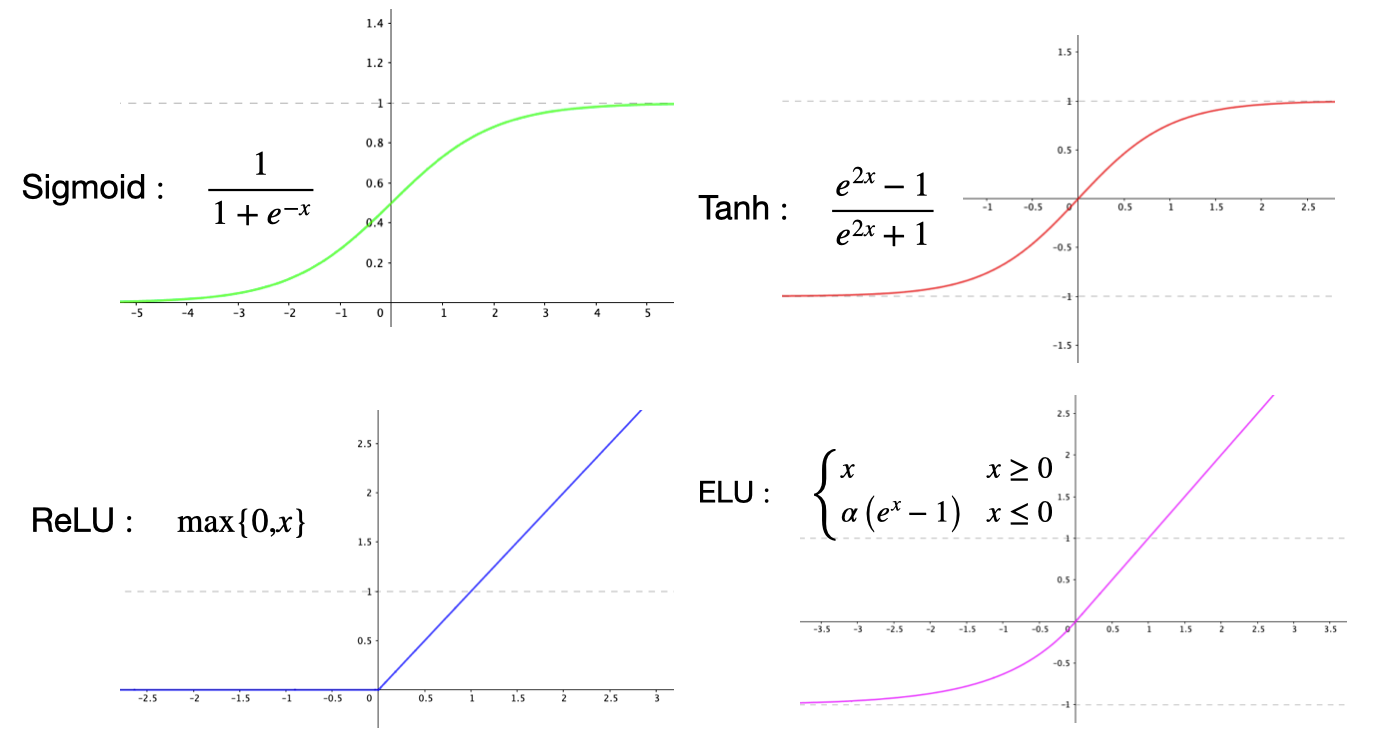
\includegraphics[width=.7\linewidth]{Pics/02_Theory/activation_functions.png}
    \caption{Typical activation functions used in NNs. The dotted grey lines represent the values of -1 and 1.}
    \label{fig:activation_functions}
\end{figure}

The size and layout of a NN is called the network architecture. The simplest type of NN architecture is the ANN. An example of a very simple ANN with only 2 input values for each observation, and binary outputs given in XX. 

\subsection{Decomposition Methods}\label{tex:decomp_methods}